%- HandOut Flag -----------------------------------------------------------------------------------------
\newif\ifHandout
%	\Handouttrue  %uncomment for the printable version

%- D0cum3nt ----------------------------------------------------------------------------------------------
\documentclass[beamer,handout,10pt]{standalone}   
\ifHandout
	\setbeameroption{show notes} %print notes   
\fi

	
%- Packages ----------------------------------------------------------------------------------------------
\usepackage{custom-style}
\usepackage{math}

%--Beamer Style-----------------------------------------------------------------------------------------------
\usetheme{toninus}








%--------------------------------------------------------------------------------------------------
%- D0cum3nt ----------------------------------------------------------------------------------------------------------------------------------
\begin{document}
%------------------------------------------------------------------------------------------------

%------------------------------------------------------------------------------------------------
\begin{frame}{Singular Reduction: Roadmap}
	%
	\begin{block}{Data:}
			\begin{itemize}
				\item A \emph{constraint set} $N$ (possibly singular),
				\item An infinitesimal action preserving $N$.
			\end{itemize}
	\end{block}
	%
	\vfill
	\pause
	%
	\begin{block}{Goal:}
		\begin{itemize}
			\item Obtain a "reduced" observables algebra out of the data.
		\end{itemize}
	\end{block}
	%
	\vfill
	\pause
	%
	\begin{block}{Strategy:}
		\begin{enumerate}
			\item Define smooth fields/forms \emph{tangent to $N$},
			\item define smooth fields/forms \emph{vanishing along $N$},
			\item define \emph{reducible fields} requiring the preservation of the vanishing objects,
			\item define \emph{reducible forms} requiring their conservation w.r.t. the infinitesimal action,
			\item define \emph{reducible and vanishing observables},
			\item \textbf{quotient}
		\end{enumerate}
	\end{block}






\end{frame}
\note[itemize]{
	\item
}

%------------------------------------------------------------------------------------------------


%------------------------------------------------------------------------------------------------
\begin{frame}[shrink]{Smooth objects on a singular set}
	Consider $N$ closed subset of $M$.
	\vfill
	\pause
	\begin{defblock}
	 $I_N$ = ideal of smooth functions vanishing over $N$.
	\end{defblock}
	\vfill
	\pause

	\begin{columns}[T]
		\setlength{\belowdisplayskip}{5pt}
		\begin{column}{.65\linewidth}
			%
			\centering \it
				\begin{defblock}[v.f tangent to $N$]
					\begin{displaymath}
						\X_N(M):=
						\left\lbrace
							v \in \X(M)
						~\Big\vert~
							\L_v(I_N) \subseteq I_N
						\right\rbrace
					\end{displaymath}
				\end{defblock}
				\begin{defblock}[v.f vanishing on $N$]
					\begin{displaymath}
						I_\X(N):=
						\left\lbrace
							v \in \X(M)
						~\Big\vert~
							\L_v(C^\infty(M)) \subseteq I_N
						\right\rbrace
					\end{displaymath}				
				\end{defblock}				
		\end{column}	
		%
		%
		\begin{column}{.35\linewidth}
			\centering 
			\includestandalone[width=0.8\textwidth]{Pictures/Figure_VfTangentN}			
		\end{column}	
	\end{columns}			
	%	
	\pause

				%

				%	
		\begin{tcolorbox}[
		enhanced,frame hidden,borderline={0.5pt}{0pt}{blue},
		arc=5pt,colback=white,
		colbacktitle=white,]
			\color{blue}{\textbf{Lem}:} If $N$ is smoothly embedded,  $\X(N)\cong {X_N(M)}/{I_\X}$.
		\end{tcolorbox}

		\pause

		\begin{defblock}[Differential form vanishing on $N$]
			\begin{displaymath}
				I_{\Omega(N)}:=
				\left\lbrace
					\alpha\in\Omega^k(M
				~\left\vert~
					\begin{array}{l r}
						k\geq 0,~		\\		
						\alpha(u_1,\ldots,u_k) \in I_N & \forall u_i \in\X_N(M)
					\end{array}
				\right\rbrace\right.
			\end{displaymath}
		\end{defblock}

\end{frame}
\note[itemize]{
 \item $N$ is not a submanifold in general. An example is $N=\mu^{-1}(0)$ for a certain smooth map $N$.
 \item observe that if $N$ is a smooth embedded submanifold, one has that $\X(N)\cong \frac{X_N(M)}{I_\X}$  

}
%------------------------------------------------------------------------------------------------



%------------------------------------------------------------------------------------------------
\subsection{Multisymplectic singular reduction}
\begin{frame}{Reducible smooth objects \quad \small (w.r.t. $N$ and $\g\curvearrowright M$)}
	Consider $\g \curvearrowright M$ by vector fields tangent to $N$ % \hfill( fond. distribution $\underline{\g}\subseteq \X_N(M)$)
	\\
	\vfill
	Denote by :  
	\hspace{1em} $\underline{\g}\subseteq \X_N(M)$ the fundamental distribution,
	\\
	\hspace{6.5em}  $\X_g$ the $C^\infty$-module generated by $\underline{\g}$.
	\\
	\vfill
	\begin{defblock}[Reducible v.fields ]
			\begin{displaymath}
				\X(M)_{[N]} :=
				\left\lbrace
					v \in \X(M)
				~\left\vert~
					\begin{array}{l}
						\L_v (I_N) \subseteq I_N	\\		
						\L_v (\X_g) \subseteq \X_g + I_\X
					\end{array}
				\right\rbrace\right.
			\end{displaymath}
%			\blfootnote{
%			 $\X_g$ = $C^\infty(M)$-module generated by the fundamental distribution.
%			}	

	\end{defblock}	
	%
	\pause
	%
	\begin{defblock}[Reducible forms ]
		\begin{displaymath}
			\Omega(M)_{[N]} :=
			\left\lbrace
				\alpha \in \Omega(M)
			~\left\vert~
				\begin{array}{l r}
					\L_\underline{\xi} \,\alpha \in I_{\Omega(N)}	\\		
					\iota_\underline{\xi} \,\alpha \in I_{\Omega(N)}	& \forall \xi \in \g				\end{array}
			\right\rbrace\right.
		\end{displaymath}	
	\end{defblock}	
	%
	\pause
	\vfill
	%
	Let $(M,\omega)$ be a $k$-plectic manifold
	\begin{defblock}[Reducible Hamiltonian forms]
		\begin{displaymath}
			(\Omega(M)_{ham}^{n-1})_{[N]} :=
			\left\lbrace
				\alpha \in \Omega(M)_{ham}^{n-1}
			~\left\vert~
				\begin{array}{l r}
					\alpha \text{ is a reducible form} \\
					\vHam_\alpha \text{ is a reducible v.field}
				\end{array}
			\right\rbrace\right.
		\end{displaymath}	
	\end{defblock}		

	
\end{frame}
\note[itemize]{
 \item $\g\curvearrowright M$ by vector field tangent to $N$ means that $\underline{\xi}\in\X_n(M) \forall \xi \in \g$
 \item Spelling out the definition: reducible vector fields are 
 \\i) v.f. tangent to N 
 \\ii) such that their commutator with any $\underline{\xi}$ lies in $\X_\g$ along $N$.
 \item more algebraically, they stabilize both $I_N$ and $\X_g + I_\X$.
 \item observe that $\L_v I_\X \subseteq I_\X$ since , $\forall u \in I_\X$ $\forall f \in C^\infty(M)$ one has\\
 $(\L_v u) f = \L_{[v,u]} f = \L_v\L_u f - \L_u\L_v f \in I_N$
 \item
}
%------------------------------------------------------------------------------------------------

%------------------------------------------------------------------------------------------------
\begin{frame}\frametitle{Hierarchy of auxiliary constructions}
	\begin{minipage}{\textwidth}
	\centering
	\scalebox{.65}{
	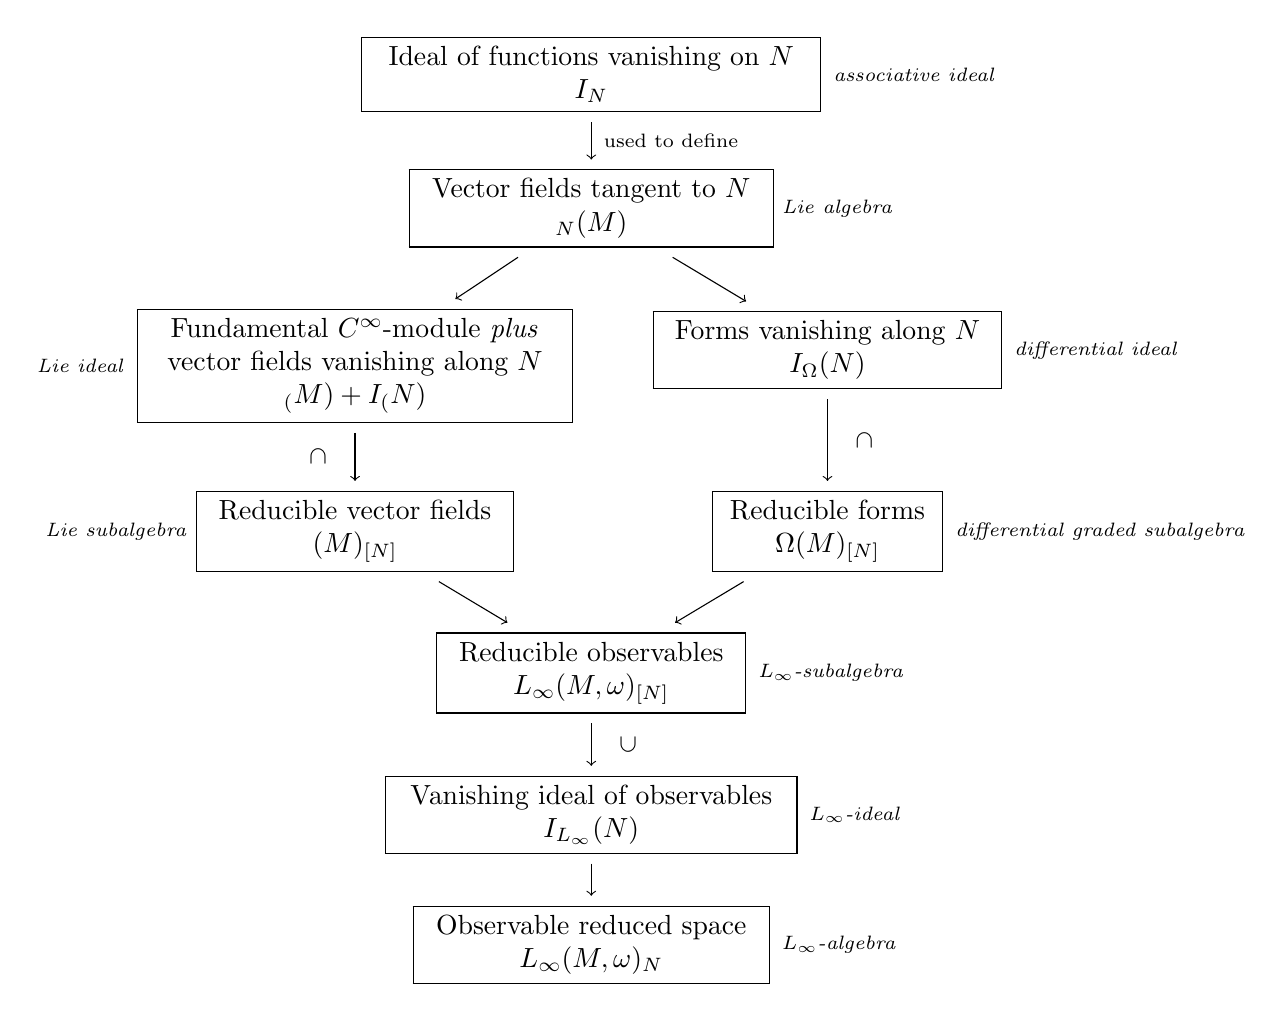
\begin{tikzpicture}
		\node (A) at (0,10.0) {\fbox{\parbox{5.6cm}{\centering Ideal of functions vanishing on $N$ \\ $I_N$}}};
		\node (B) at (0,8.3) {\fbox{\parbox{4.4cm}{\centering Vector fields tangent to $N$ \\ $\X_N(M)$}}};
		\node (C) at (3,6.5) {\fbox{\parbox{4.2cm}{\centering Forms vanishing along $N$ \\ $I_\Omega(N)$}}};
		\node (D) at (3,4.2) {\fbox{\parbox{2.7cm}{\centering Reducible forms \\ $\Omega(M)_{[N]}$}}};
		\node (E) at (-3,6.3) {\fbox{\parbox{5.3cm}{\centering Fundamental $C^\infty$-module \emph{plus} \\ vector fields vanishing along $N$ \\ $\X_\g(M)+I_\X(N)$}}};
		\node (E') at (-3,4.2) {\fbox{\parbox{3.8cm}{\centering Reducible vector fields \\ $\X(M)_{[N]}$}}};
		\node (F) at (0,2.4) {\fbox{\parbox{3.7cm}{\centering Reducible observables \\ $L_\infty(M,\omega)_{[N]}$}}};
		\node (G) at (0,0.6) {\fbox{\parbox{5.0cm}{\centering Vanishing ideal of observables \\ $I_{L_\infty}(N)$}}};
		\node (H) at (0,-1.05) {\fbox{\parbox{4.3cm}{\centering Observable reduced space \\ $L_\infty(M,\omega)_N$}}};

		\draw[->] (A)-- node[right=1pt]{{\scriptsize used to define}} (B);
		\draw[->] (B)-- (C);
		\draw[->] (C)-- node[right=.25cm]{\rotatebox{-90}{\small $\subset$}} (D);
		\draw[->] (B)-- (E);
		\draw[->] (D)-- (F);
		\draw[->] (E)-- node[left=.25cm]{\rotatebox{-90}{\small $\subset$}} (E');
		\draw[->] (E')-- (F);
		\draw[->] (F)-- node[right=.25cm]{\rotatebox{90}{\small $\subset$}} (G);
		\draw[->] (G)-- (H);

		\node[right=2.95cm] at (A) {\scriptsize\emph{associative ideal}};
		\node[right=2.30cm] at (B) {\scriptsize\emph{Lie algebra}};
		\node[right=2.25cm] at (C) {\scriptsize\emph{differential ideal}};
		\node[right=1.5cm] at (D) {\scriptsize\emph{differential graded subalgebra}};
		\node[left=2cm] at (E') {\scriptsize\emph{Lie subalgebra}};
		\node[left=2.8cm] at (E) {\scriptsize\emph{Lie ideal}};
		\node[right=2cm] at (F) {\scriptsize\emph{$L_\infty$-subalgebra}};
		\node[right=2.65cm] at (G) {\scriptsize\emph{$L_\infty$-ideal}};
		\node[right=2.3cm] at (H) {\scriptsize\emph{$L_\infty$-algebra}};
	\end{tikzpicture}
	}
	\end{minipage}
\end{frame}
\note[itemize]{
 \item
}

%------------------------------------------------------------------------------------------------

%------------------------------------------------------------------------------------------------
\begin{frame}{Multisymplectic observable reduction}
	\begin{defpropblock}[Reducible $L_\infty$-observables]
		Is the {\color{blue!70!black}$L_\infty$-subalgebra} of $L_\infty(M,\omega)$ given by
		\begin{displaymath}
			L_\infty(M,\omega)_{[N]}^k :=
			\begin{cases}
				\Omega^{n-1-k}(M)_{[N]} 
				\qquad\text{\color{gray}\small (reducible forms) }
				& \text{if } n-1\leq k < 0 \\
				(\Omega(M)_{ham}^{n-1})_{[N]} 
				\quad
				\text{\color{gray}\small (reducible hamiltonians) }
				& \text{if } k = 0 \\
				0 & \text{if } k > 0
			\end{cases}
		\end{displaymath}
	\end{defpropblock}
	%
	\pause
	%
	\begin{defpropblock}[Vanishing $L_\infty$-observables]
		Is the {\color{blue!70!black}$L_\infty$-ideal} of $L_\infty(M,\omega)_{[N]}$ given by
		\begin{displaymath}
			I_{L_\infty(M,\omega)} :=
			\left\lbrace
				\alpha \in L_\infty(M,\omega)_{[N]}
			~\left\vert~
				\begin{array}{l l}
					\alpha(v_1,\dots,v_k) \in I_N  \quad \forall v_i \in \X_N &
					\text{if}~ \alpha \in \Omega^k \\
					\vHam_\alpha \in \X_\g + I_\X &
					\text{if}~ \alpha \in \Omega^{n-1}
				\end{array}
			\right\rbrace\right.
		\end{displaymath}
	\end{defpropblock}
	%
	\pause
	%
	\begin{thmblock}[Blacker - M. - Ryvkin]%[Reduced $L_\infty$-algebra of observables]
		The reduction of $L_\infty(M,\omega)$  with respect to $\g\curvearrowright (N\subset M)$ is the %$L_\infty$-algebra
		quotient
		\begin{displaymath}
					L_\infty(M,\omega)_N = \frac{L_\infty(M,\omega)_{[N]}}{I_{\L_\infty}(N)}~.		
		\end{displaymath}
	\end{thmblock}

\end{frame}
\note[itemize]{
 \item The graded vector space underlying the reduced $L_\infty$-algebra $\Ham_\infty(M,\omega)_N$ is explicitly given by
\begin{displaymath}
	\Ham_\infty(M,\omega)_N =
	\frac{
		\left\lbrace
			(\alpha,v) \in \Omega(M){[n{-}1]}\oplus\X(M)
		~\left\vert~
			\begin{array}{l l}
				\iota_v \omega = -\d \alpha^{(0)} &
				\\
				\iota_\xi \alpha \in I_{\Omega}(N) &
				\\
				\L_\xi\alpha \in I_{\Omega}(N)
				&
				\\
				\L_\xi v \in \fgmodule +\vanvf
				&~\forall \xi \in \g 
				\\
				v \in \X_N(M)
				&
			\end{array}
		\right.
		\right\rbrace
	}{
		\left\lbrace
			(\alpha,v) \in \Omega(M){[n{-}1]}\oplus\X(M)
		~\left\vert~
			\begin{array}{l}
				\alpha \in I_{\Omega}(N)
				\\
				v \in \fgmodule +\vanvf
			\end{array}
		\right.
		\right\rbrace
	}~.
\end{displaymath}
}
%------------------------------------------------------------------------------------------------

%------------------------------------------------------------------------------------------------
\begin{frame}{Singular reduction (Conclusions)}
		  \centering 
	\emph{Reduction of states vs.\ reduction of observables}
	\vfill
	\begin{minipage}{.7\textwidth}
	\hspace{-.4cm}
	\begin{tikzpicture}
		\draw (-4,-2.5) rectangle (4,2.5);
		\draw (-4,0) -- (4,0);
		\draw (0,-2.5) -- (0,2.5);

		\draw node[align=center] at (-2,1.25) {symplectic\\ reduction};
		\draw node[align=center] at (2,1.25) {multisymplectic\\ reduction};
		\draw node[align=center] at (-2,-1.25) {\'{S}niatycki--Weinstein,\\Dirac,\\Arms--Gotay--Jennings\\ reduction};
		\draw node[align=center] at (2,-1.25) {\color{UniGreen}$L_\infty$ reduction};

		\draw node[align=center] at (2,2.85) {\color{UniGreen}\emph{higher}};
		\draw node[align=center] at (-2,2.85) {\emph{lower}};

		\draw node[align=right] at (-4.7,1.25) {\emph{states}};
		\draw node[align=right] at (-5.13,-1.25) {\color{UniGreen}\emph{observables}};
	\end{tikzpicture}
	\end{minipage}


	
	\pause
			\vfill
		  \centering 
		  {\Huge\color{red} 
		  \emph{Thank you for your attention!}}
\end{frame}
\note[itemize]{
 \item Consider $N=\mu^{-1}(0)$ to be regular (smooth embedding)
		\vspace{.5em}
		\begin{table}[]
			\begin{tabular}{ccc}
			Multisymplectic               &                      & Multisymplectic                  \\
			regular                       & $\equiv$             & singular                \\
			reduction & & reduction
			\end{tabular}
		\end{table}	

		\item
			Consider $\omega$ to be $1$-plectic
			\vspace{.5em}
			\begin{table}[]
				\begin{tabular}{ccc}
				Multisymplectic               &                      &  Sniaticky--Weinstein                  \\
				singular                       & $\cancel\equiv$             & singular                \\
				reduction & & reduction
				\end{tabular}
			\end{table}	

			(but $\exists$ a canonical Poisson algebra morphism) 
 
}
%------------------------------------------------------------------------------------------------









%------------------------------------------------------------------------------------------------
\ifstandalone
\begin{frame}[t,shrink]{Extended Bibliography}
	\cite{Blacker20}
	\bibliographystyle{alpha}
	\bibliography{bibfile}
\end{frame}
\fi
%------------------------------------------------------------------------------------------------

%------------------------------------------------------------------------------------------------
\end{document}